\section{Results}
\newcommand{\Ftest}[4]
{\textit{F}(#1,#2) = #3, \textit{p}$=$
#4}
\subsection{Hit Rate}
First, a significant main effect of LSAS showed that higher LSAS scores were associated with higher hit rates in general, \Ftest{1}{684}{4.74}{.030}. A significant interaction between LSAS and emotion further revealed that the higher hit rate associated with social anxiety was emotion-specific, \Ftest{3}{684}{4.62}{.003}. Specifically, the positive association between LSAS and hit rates was only shown for angry, \Ftest{1}{509.53}{11.88}{.001}, and fearful faces, \Ftest{1}{509.53}{5.97}{.015}, but not for happy, \textit{p}=.856, or sad faces, \textit{p}= .390. Second, a significant main effect of mask use was observed, \Ftest{1}{684}{103.07}{.001}. Participants generally identified facial emotions less correctly in masked conditions. There was also a significant interaction between mask use and emotion, \Ftest{3}{684}{15.23}{.001}. A post-hoc test with Bonferroni correction showed that the negative impact of mask use on hit rate was only shown in fearful, happy, and sad faces, \textit{p}s <.001, while angry faces had a similar hit rate in both the masked and unmasked conditions, \textit{p}=1.000. This suggested that participants mainly relied on the regions around the eyes to identify angry faces while recognizing other emotions required information in the lower face. Thirdly, a significant main effect of emotion was also revealed, \Ftest{3}{684}{55.35}{.001}, and the Bonferroni-corrected post-hoc test showed that hit rates significantly differed among four emotions, with the highest hit rates for happiness, then fear, followed by anger, and lastly sadness (happiness vs. fear: \textit{p}= .005; other pairwise comparisons: \textit{p}s< .001). Contrary to our hypothesis, there was neither a significant interaction between LSAS and mask use, \Ftest{1}{684}{0.00}{.998}, nor a LSAS x mask use x emotion interaction, \Ftest{3} {684}{0.35}{.789}.
\subsection{Eye Movement Patterns During Facial Emotion Recognition}
The two representative eye movement patterns (Pattern A and Pattern B) during facial emotion recognition found by clustering in EMHMM are shown in Figure~\ref{fig:gearhead}. The two patterns were significantly different, as the data from participants adopting Pattern A were more likely to be generated by Pattern A HMM than Pattern B HMM, \textit{t}(449) = 14.49, \textit{p}< .001, and vice versa for data from participants adopting Pattern B, \textit{t}(253) = 9.68, \textit{p}< .001. In Pattern A, a scan path mostly started with a fixation at a broad region that centered at the midpoint between two eyes and spread from the eyebrows and above the upper lip (red, 97\%), with small occasions to start at the forehead region (magenta, 2\%) or at a smaller region only covering the eye and the nose regions (blue, 1\%). After the fixation to the broad region (red), the path typically switched to narrower regions covering the nose and eye regions (red to blue, 47\%) or eye region only (red to green, 48\%), and then mostly remained at the same regions. In contrast, in Pattern B, the scan path typically started at a region that centered at the nose tip and spread from the brow ridge to the mouth region (red, 68\%), with probabilities of starting at a smaller region centered at the left cheek of the model (blue, 15\%; magenta, 12\%) or small occasions that start at a broad region that centered the mouth (green, 5\%). Participants tended to remain at the same fixation region after making their first fixation to the nose-tip-centered region (red to red, 100\%).  In sum, Pattern A represented a more eye-centered viewing strategy when identifying facial emotions, whereas Pattern B described a more nose-centered strategy. Thus, we termed Pattern A the “eye-centered strategy” and Pattern B the “nose-centered strategy”. Afterward, we examined whether social anxiety was associated with the differences in the tendency to use a more eye-centered or a nose-centered strategy across conditions (quantified by the A-B scale).
The mixed-effect model showed a significant main effect of mask use, \Ftest{1}{602}{1089.52}{.001}, with an overall increase in using eye-centered strategy associated with mask use. There was no significant main effect of LSAS, \Ftest{1}{82}{0.32}{.570}, or emotion, \Ftest{3}{602}{1.41}{.240}. There was also no significant interaction effect: the interaction between LSAS and mask use, \Ftest{1}{602}{3.47}{.063}; the emotion x LSAS interaction, \Ftest{3}{602}{0.17}{.918}; the emotion x mask use interaction, \Ftest{3}{602}{1.00}{.391}; the interaction between emotion, mask use, and LSAS, \Ftest{3}{602}{0.59}{.619}. This indicated that participants with different social anxiety levels adopted a similar eye movement strategy during emotion recognition across emotion and mask use conditions. 
\begin{figure}[h!] 
\caption{\label{fig:gearhead} The Two Representative Patterns Found in EMHMM}
\centering
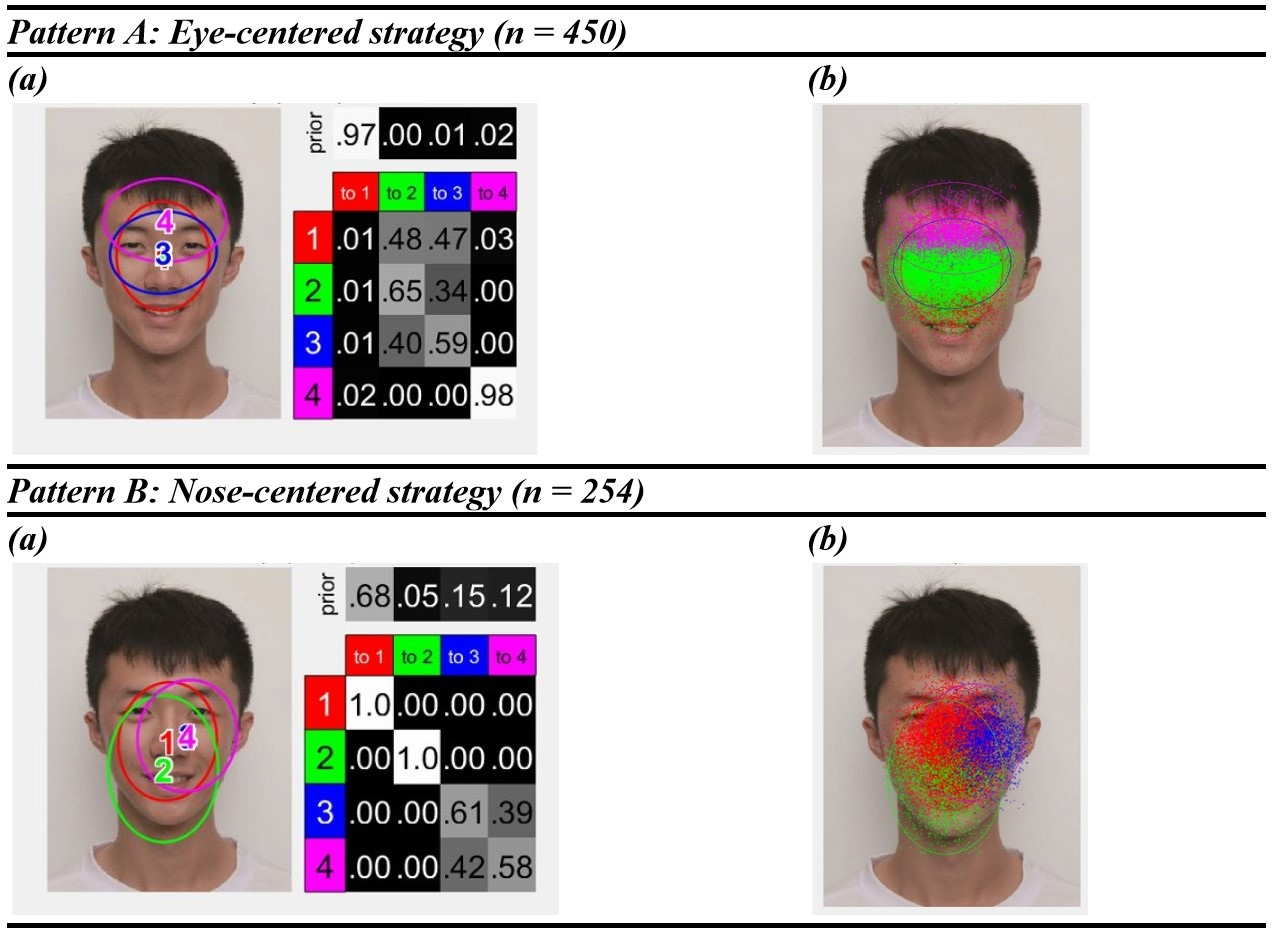
\includegraphics[width=0.7\textwidth]{frog_1.jpg}
\caption*{Notes. (a) The representative hidden Markov model. The ellipses on the left show the ROIs as 2-D Gaussian emissions. The table on the right shows the priors (the probabilities that a fixation sequence starts from the ellipses) and the transition probabilities from one ROI to another in the sequence. (b) The actual assignment of fixations to each ROI.}
\end{figure}
